\chapter{Three issues in the FDI literature}
\label{chap:literature_issues}

\section{Estimating countries' demand for FDI}

The IPE literature on the political determinants of FDI has overwhelmingly
focused on what MNCs demand from countries, not what countries demand from MNCs.
In this literature, politics matters, but only in terms of what political
factors make countries attractive to MNCs. As Jensen states in the introduction
of \textit{Nation-states and the multinational corporation}:

\begin{quote}
  Which government policies prove beneficial to multinational corporations?
  Which political institutions provide multinational corporations with credible
  commitments to these market-friendly policies? These emerge as the central
  questions of this book.
\end{quote}

Other scholars share the same line of inquiry \citep{Ahlquist2006, Busse2007,
  Buthe2008, Li2003}. In their theoretical argument, the central dynamics of the
negotiation between countries and MNCs is that FDI is mobile before MNCs make
the investment on the ground but immobile after. Since the cost of relocation is
higher the more investment MNCs commit, the original bargain between the host
country and the MNC become increasingly obsolete as the host country can alter
the original bargain at the expense of the MNC, knowing that relocating would
cost the MNC dearly. Therefore, certain political institutions, such as
democracy, veto players, and federalism, increase FDI inflow because they can
credibly commit not to change their policies \textit{ex post}, and are thus
attractive to MNCs.

In theorizing FDI inflow largely as a function of MNCs' preference, the FDI
literature implicitly assumes that countries are eager to receive as much FDI as
possible. 
Contrary to the assumption that countries are largely open to FDI and that FDI
inflow is mainly driven by MNCs' preference, a historical and comparative
examination of FDI policies makes it clear that countries have at best had a
mixed attitude towards foreign capital, especially when they are at an early
stage of development and are a net recipient of FDI. As they receive more than
sending FDI, countries at this stage tend to be more concerned about the
ramifications of FDI on the domestic economies than with protecting the interest
of their business abroad. As an example, consider the FDI policies of a rapidly
industrializing country, who within 30 years of intense globalization had
overtook incumbent industrial giants to become the factory of the world and the
largest recipient of FDI. I am writing, of course, about the U.S. at the turn of
the 20\textsuperscript{th} century. From 1879 to 1909, the U.S. transformed
itself from an economy dominated by agriculture (53\%) to one dominated by
industry (62\%). Its population doubled from 40 million in 1870 to 92 million in
1910. In 1914, it surpassed Britain's industrial output, producing more than one
third of the global output. Advances in communication and transportation
technologies ushered in unprecedented movement of people and capital---the
so-called first globalization era \citep{Estevadeordal2003}. During this period,
the U.S. was the most popular destination for global capital and the world's
greatest debtor nation \citep[part II]{Wilkins1989}.

Despite its staunch advocacy for liberal FDI policies nowadays, the U.S had at
best a mixed attitude towards attitude when it was a net recipient of FDI. While
American business were aware of the benefits of FDI (capital funding risky and
large scale investment in mining and railroad, potential for technologies), they
become hostile towards FDI when they feel like there were adequate capital at
home, that the tribute paid to foreign owners are odious, that foreign
managements demanding restructuring do not understand American problems and may
ruin the railroad industry, that foreign ownership of land touches an emotional
nerve when people feel that land is a limited resource and that ``our land''
should not be controlled by European absentee owner. lead to state legislation
forbiding nonresident alien ownership of land, tighten regulation around foreign
banks, insurance companies, and mortgage lenders. 1913 federal forbid foreign
citizens to be directors of U.S. national banks, foreign citizens can only buy
share of U.S. banks if they are willing to have U.S. citizen as their
representatives on the board \citep{Wilkins1989}.

A similarly restrictive attitude towards FDI characterized South Korea's
policies during its industrializing period. After almost half a century of
oppression under Japanese colonialism, South Korea was deeply averse to a large
foreign presence in their economy. This nationalistic impulse translated into a
host of restrictions on FDI entry and ownership. Throughout the 1960s and 1970s,
instead of keeping a small list of restricted sectors, Korea used a positive
list system that forbade FDI in all sectors except those explicitly allowed by
the government. Even in sectors that allowed FDI, majority foreign ownership was
also forbidden \citep{Thurbon2006}. Even as late as the 1980s, after mounting
internal pressure for a more liberal FDI policies, 50\% of all industries and
20\% of manufacturing industries were still closed to MNCs, and only 5\% of MNCs
in Korea were wholly owned by the foreign investor \citep{Chang2004}. On top of
these explicit restrictions, a FDI project must also be approved by numerous
agencies, including the Ministry of Trade and Industry, the Ministry of Science
and Technology, and the Ministry of Finance. The subsequent red tape and delay
further deterred MNCs from entering.\footnote{The arduous approval process for
  FDI projects is a deliberate policy choice by the Korean government and not
  the result of lacking state capacity. Indeed, as \citet{Evans1995} describes,
  Korea had a strong and autonomous state, capable of outlining and executing a
  developmental strategy for the country. Its FDI policies are an integral part
  of this strategy, as outlined in the Economic Planning Board (EPB)'s 1981
  \textit{White Paper on Foreign Investment} \citep{EconomicPlanningBoard1981}.
  Korea's policy of meticulous vetting stands in stark contrast with recent
  efforts to fast track FDI projects (often called the ``one-stop shop'')
  promoted by international organizations, e.g. in Dominican Republic
  \citep{UNCTAD2016}, Nigeria \citep{UNCTAD-Nigeria2009}, and many others.}
Instead of attracting FDI, Korea relied much more on foreign debt for its
capital need. As a result, from 1962 to 1983, FDI made up only 5.1\% of foreign
capital in Korea (author's calculation based on data reported in \citet[92,
Table 4.5]{Amsden1989}).

More importantly, countries have shown that they choose their FDI policies
strategically, being restrictive at times and enthusiastic at others, adapting
to fit their political and economic conditions. If we make blanket assumptions
about countries' preference for FDI instead of studying how it varies, we
overlook this strategic component entirely. Consider the case of China, whose
demand for FDI has ebbed and flowed dramatically over time. Before, during, and
after the period of economic reform, China's attitude towards FDI swung from
extreme hostility, to red carpet treatment, and finally chilly co-existence.
Indeed, before the 1979 economic reform, there was virtually no foreign capital
in China, and Chinese leaders took great pride in their nationalistic
self-sufficiency. They even turned down foreign aid from the International Red
Cross for the 1976 Tangshang earthquake, announcing that such disasters ``teach
the value of self-reliance and hard struggle.'' \citep{Butterfield1976}.
However, when the disastrous result of central planning and the Cultural
Revolution became apparent, especially in stark contrast with the shining
achievements of neighboring Asian tigers, China committed to Deng Xiaoping's
``open door policy'' in 1979. With the promulgation of the ``Law on Chinese
Foreign Equity Joint Ventures,'' the flood gate opened for foreign capital
\citep{Wei1996}. Throughout the reform period, China's FDI policies continuously
grew friendlier over time. In 1986, after Deng Xiaoping's famous Southern tour
to shore up support for reform, China moved from ``permitting'' to
``encouraging'' FDI, allowed wholly owned foreign enterprises, and adopted a
negative list approach that accepted FDI in all sectors unless specifically
banned. Finally, after China joined the WTO in 2001, to meet its membership
obligation China abolished various performance requirements (e.g. export ratio,
local content, technology transfers, etc.) previously imposed on foreign firms
\citep{Long2005}.

During this reform period, China did not just allowed FDI---it also favored
foreign firms over the domestic sector. While Chinese leaders continued to view
the domestic sector with suspicion, they had no problem with foreign firms,
whose main goal is to make money, not to raise political trouble. China used FDI
in special economic zones as ``laboratories of capitalism,'' experimenting
incrementally with the market economy without creating a class of indigenous
capitalists that could start challenging the state \citep{Gallagher2002}. As a
result, China created a dualist legal regime that much better protected foreign
firms than domestic ones. For example, China made a legislative commitment in
1979 and a constitutional commitment in 1982 not to expropriate from foreign
enterprises. There was no such guarantee for the domestic sector. Compared to
domestic firms, foreign businesses also seemed to enjoy fewer audits, more
favorable judgment during labor dispute, and more assistance from the government
\citep{Huang2003, Huang2011}. Indeed, during the early reform years, FDI firms
enjoyed such large benefits that even state-owned enterprises (SOEs) were eager
to form joint venture with them \citep[59]{Gu1997}.

However, as China's developmental strategy shifted to nurturing its domestic
sector into a world class competitor, its attitude towards FDI and domestic
firms reversed. In 2010, some European firms started grumbling about unfair
treatments, especially in sectors where intellectual property was important,
while others remained happy with making good money. As an observer remarked,
``China still welcomes FDI, but \ldots it is becoming more insistent on setting
the terms,'' including favoritism towards domestic firms for government
contracts, higher tax rate, or a limit on the number of non-Chinese staff
\citep{Grant2010}. By 2016, the accusations of discrimination against foreign
firms had become mainstream. A former deputy trade representative for the US
complained that foreign insurers had to apply for one license at a time, taking
six to eight months total. In contrast, Chinese rivals could submit their whole
package and got approved quicker despite claims of equal treatment from the
government. In its annual business climate survey, the American Chamber of
Commerce in China reported that, between 2015 and 2017, from 75\% to 81\% of
businesses felt that they were less welcome than before
\citep[39]{AmCham2018}.\footnote{The business climate survey first asked this
  question in 2015.} As James McGregor, former bureau chief of the Wall Street
Journal and the chairman of AmCham China, a business executive who lived in
China for more than two decades, observed \citep{Wu2016}:

\begin{quote}
  For foreign companies in China, right now is perhaps the most distressing and
  unhappy time that I have seen. \ldots They feel that the best days for foreign
  companies in China are reaching an end.
\end{quote}

In sum, the prevailing assumption in the FDI literature that all countries are eager
for FDI is untenable. Many countries, including those that eventually become staunch
supporters of liberalizing FDI policies, have held restrictive policies on FDI when
they were net recipient of FDI. More importantly, countries have shown a dynamic
preference for FDI, adapting their policies to meet their political and economic
goals.

Unfortunately, the two common empirical approaches in the literature strongly
rely on this
assumption. In the first approach, researchers build a regression model with FDI
inflow as the dependent variable and a political factor as the independent
variable of interest. The problem with this model is that it is impossible to
interpret the political factor as an attraction to MNC or as a motivator of
countries' demand for FDI. Consider \citet{Jensen2005}'s finding that federalism
is positively associated with FDI inflow. The authors interpret this correlation
as federalism constraining the whim of the central government, increasing policy
stabilities, and thus making the country attractive to MNCs. However, the
alternative explanation is that local governments in a decentralized system
compete more intensely for FDI, driving up the FDI inflow. For example, As China
decentralized in the late 1980s and early 1990s, local governments gained the
authority to approve foreign investment up to a certain size, thus able to court
MNCs without asking the central government for permission.\footnote{Similar to
  China's broader economic reform, decentralization in China's FDI policies
  happened incrementally. In 1979, China first allowed FDI in four Special
  Economic Zones, i.e. Shenzhen, Zhuhai, Shantou (near Hong Kong), and Xiamen
  (near Taiwan). As the economic benefits of FDI became clear, provinces started
  clamoring for the ability to attract FDI themselves. Therefore, in 1984, China
  allowed 14 coastal cities to approve FDI projects themselves, and in the early
  1990s, allowed inland regions to do the same. \citet{Gallagher2002, Shirk1993}
  discuss how the coalition for decentralization expanded over this period, and
  \citet{Coase2012} provides a historical account of China's economic reform
  more broadly.} In addition, local governments could keep all revenue in excess
of a quota pre-negotiated with the central government, further motivating them
to bring in MNCs as a lucrative source of tax revenue. Having both the authority
and the incentive to attract MNCs, Chinese local governments engaged in an
intense competition for MNCs. For example, while there were only 117 development
zones in 1991, the number exploded to 2700 in 1992, of which only 95 were
initiated by central ministries \citep{Montinola1995}. Far from
\citet{Jensen2005}'s argument, China's federalism did not increase FDI inflow by
producing a static policy environment that MNCs like. On the contrary,
federalism incentivized Chinese local governments to demand FDI, fostering local
policy experiments that were anything but stable.\footnote{A very similar
  account of decentralization causing provincial demand and competition for FDI
  happened in Vietnam as well \citep{Malesky2004c}.}

In the second approach, researchers estimate MNCs' preference using discrete
choice model. The dependent variable is the MNC's choice of a location over all
the others, and the independent variable of interest is a characteristic of the
location \citep{Arauzo-Carod2010}. In discrete choice model, the assumption is
that all locations are available for the MNC to pick and choose, effectively
ruling out the possibility that the host country can decline the MNC's
investment proposal. Such an assumption is unfounded. For example, in 2007, Da
Nang, a central province of Vietnam known for its public governance quality,
turned down \$2.5 billion dollars from a Taiwanese-Japanese steel factory and a
Japanese paper pulp factory for environmental concern \citep{HDung2007}. In
2014, even during tough times, when Da Nang's and Vietnam's FDI inflow was
merely half of the previous year, Da Nang's attitude towards FDI remained
selective. According to Mr. Lam Quang Minh, Director of Da Nang's investment
promotion agency, Da Nang declined a \$200-million Hong Kong textile factory and
a 30-hectare Korean dyeing facility, even when ``these [refusals] have
contributed to Da Nang's lackluster FDI attraction recently''
\citep{HaiChau2015}. While Da Nang is the most well-known for its selectiveness,
other Vietnamese provinces have also refused large FDI projects that use too
much land, exploit natural resources, or cause environmental concerns
\citep{QuocHung2015}.

Unlike the FDI literature, the broader field of IPE has recognized that
countries' preferences remain an important force even in a globalized era.
Indeed, despite early pessimism about countries engaging in a race to the bottom
to attract footloose global capital, scholars have shown substantial variation
in countries' trade, welfare, environmental, and fiscal policies
\citep{Drezner2001}. The FDI literature has lagged behind in this aspect.

\subsection{Current approaches to estimate countries' demand for FDI}

Recognizing this gap in the FDI literature, \citet{Pinto2013} and \citet{Pandya2016}
recently broke ground in this area. Similar to the rich IPE literature in
international trade, these studies argue that countries' demand for FDI varies
according to FDI's distributive effect on their domestic constituencies
\citep{Broz2001, Milner2005a}. In this theoretical framework, labor supports FDI
because foreign firms bring capital that increases the demand for labor and
raises productivity, both of which lead to higher wage. On the other hand,
domestic firms oppose FDI because foreign firms compete for local labor, inputs,
and markets. Both \citet{Pinto2013} and \citet{Pandya2016} formulate their
theories as a variant of this labor-vs-business tension, which surfaces in the
former work as left-vs-right governments, and in the latter as
democratic-vs-authoritarian regimes.

While these pioneering works have enriched our understanding of the relationship
between politics and FDI, their empirical approaches do not satisfactorily
measure countries' demand for FDI, leaving their theoretical arguments untested.

Consider \citet{Pinto2013}'s approach. The author controls for economic and
institutional factors that affect FDI flow into a country, then claims that
what's left in the residual is the country's demand for
FDI.\footnote{Specifically, the estimation of FDI openness involves two steps.
  First, the author runs a gravity model explaining bilateral FDI flows,
  estimating the intercept as the host country-year fixed effect. Second, this
  fixed effect is then regressed on several economic and endowment factors of
  that country-year (i.e. GDP, GDP per capita, average school years, arable
  land). The residual in the second stage is considered the country's ``FDI
  openness'' in that year.} For this approach to be valid, every economic,
institutional, and endowment factors that affect FDI flow has to be controlled
for, leaving only the country's demand in the error term. This claim is much
stronger than the common assumption of exogenous error, which is valid as long
as the omitted factors are uncorrelated with the independent variable of
interest. Framed substantively, since the residual is likely to contain more
than just the country's demand for FDI, if we observe an abnormally high level
of FDI, we do not know whether it is because the country welcomes FDI or because
MNCs find something attractive in the country.\footnote{In addition, this
  approach requires data on bilateral FDI flow, ideally disaggregated by
  sectors. Therefore, this approach is limited to OECD countries only
  \citep{Pinto2008}. During the period the authors study, 1980-2000, OECD
  countries account for 95\% of global FDI outflow and 90\% of inflow. However,
  since then the role of the developed world in global FDI has declined sharply,
  reducing to 60.8\% of outflow and 40.6\% of inflow in 2014
  \citep{UNCTAD2015}.}

In contrast to \citet{Pinto2013}'s statistical approach, \citet{Pandya2014,
  Pandya2016} attempts to find a proxy for countries' demand for FDI. The author
uses the annual US Investment Climate Reports to construct the number of
industries that have foreign ownership restrictions or face investment
screening. The advantages of this measurement are its ease of interpretation and
its availability for many countries. However, two problems remain. First, adding
up the raw count of restricted industries is not appropriate because industries
are not the same. For example, given the reach of the banking sector into all
corners of the economy, a country's opening up its financial industry indicates
much more FDI-friendliness than, say, allowing foreign furniture makers to set
up shops. Since the theoretical argument is driven by FDI's distributive effect,
we must not ignore the varying impact of FDI across sectoral constituencies.

Second, according to the coding rule, an industry is coded as free if there is
no mention of restriction. However, when there is little FDI, US Investment
Climate Report may find it not worth mentioning and does not report the
restrictions. Therefore, ``zero restriction'' in the dataset can either mean
that a country is very closed or very open to FDI. This concern is not
hypothetical. Figure \ref{fig:china_fdi_restriction} shows that, following the
coding of the US Investment Climate Reports, China seemed 100\% open to FDI up
until 1986 when it started imposing restrictions. The reality is the opposite.
Prior to 1986, only limited FDI was allowed as joint-venture in Special Economic
Zones (SEZ). The year of 1986 was, in fact, the first time China allowed any
wholly owned FDI outside of SEZs.

\begin{figure}[tbp] \centering
  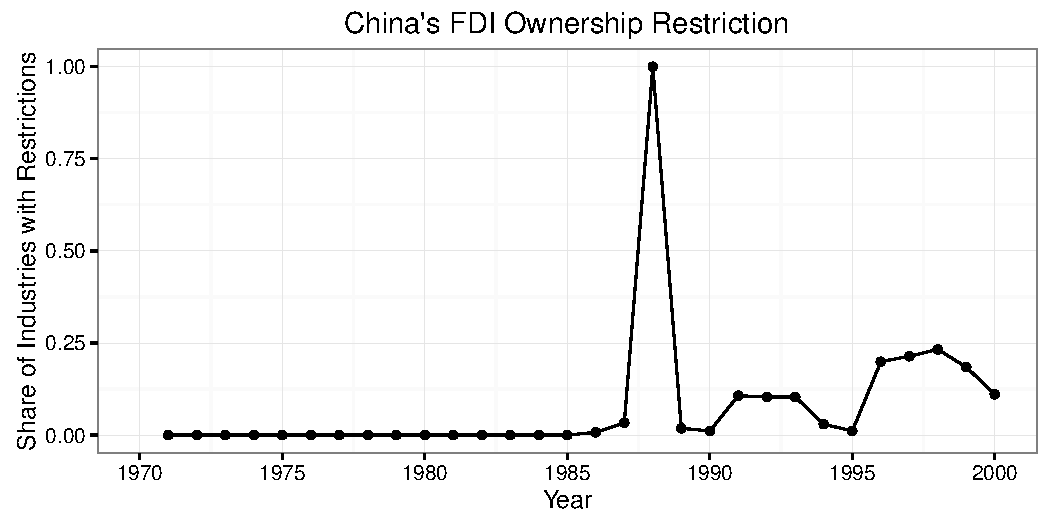
\includegraphics[width=0.8\textwidth,keepaspectratio]{china_fdi_restriction}
  \caption[China's FDI ownership restriction.]{China's FDI ownership
    restriction, as coded in \citet{Pandya2010}. Prior to 1986, FDI in China was
    limited to few experimental Special Economic Zones, and thus not mentioned
    in US Investment Reports. The sharp spike in 1988 also does not seem to
    correspond to any actual change in policy, and likely another artifact of
    reporting. (See \citet{Zebregs2002} for a historical overview of China's FDI
    policy.)}
  \label{fig:china_fdi_restriction}
\end{figure}

The two-sided matching model circumvents these thorny measurement issues by
modeling countries' demand for FDI directly. Intuitively, if we observe that a
country welcomes certain firms to invest but not others, we can compare the
characteristics of the invited and the uninvited firms to infer that country's
preference for FDI.

\section{Estimating countries' preference for types of FDI}

In addition to estimating countries' demand for FDI, we should also examine
countries' preference for different types of FDI. Indeed, while the Political
Science literature has focused almost exclusively on the quantity of FDI,
treating all FDI as one homogeneous flow of capital, policy makers seem to pay
much more attention to distinguishing its types. Commenting on the role of
International Investment Agreements, \citet{UNCTAD2015} says, ``Today,
increasing the quantity of investment is not enough. What matters is its
quality, i.e. the extent to which investment delivers concrete sustainable
development benefits.'' Governments in developing countries all offer various
forms of tax incentives and fee waivers to attract FDI that invests in a remote
region, brings new technology, or focuses on exporting \citep{Ricupero2000}. For
example, since 2006, China's official FDI policy has been ``quality over
quantity,'' promoting FDI with intense R\&D in high-productivity sectors
\citep{Guangzhou2011}.

Examining the evolution of countries' FDI policies reveal sophisticated
preference for types of FDI.

In addition to restricting FDI entry, Korea also made sure that they attracted
the types of FDI that fit their developmental strategy. The authority over FDI
policies was thus given to the Economic Planning Board (EPB), Korea's umbrella
developmental agency in charge of developing and implementing a series of
five-year plans. In its 1981 \textit{White Paper on Foreign Investment}, the EPB
displayed a sophisticated understanding of the costs and benefits of FDI and
showcases its vision for how FDI might contribute to Korea's developmental goal.
The White Paper recognized that FDI could benefit Korea by bringing capital, job
creation, potential technological upgrading, and better balance of payment. At
the same time, it cautioned that MNCs might engage in transfer pricing, demand
distortionary import-export protection, crowd out domestic investors, delay
domestic technological capability, and even exert political influence on the
government \citep[50-64, quoted in \citet{Chang2004}]{EPB1981}.\footnote{It is
  remarkable that the White Paper touched on all arguments in academic circles,
  showing that the Korean government paid close attention to the effects of
  FDI.} Therefore, in pursuing developmental strategy based on national
ownership, the EPB heavily restricted MNCs that targeted the local market,
especially in labor-intensive sectors where the government believed there were
domestic alternatives. On the other hand, the EPB prioritized FDI projects that
were export-oriented and too technically complex for Korean producers. In
addition, the EPB strongly preferred MNCs that were willing to improve the
capabilities of Korean producers by procuring from local suppliers, transferring
technologies to local partners, providing access to foreign markets, even
divesting the foreign-held equities to the Korean partner after a specified
date. Indeed, of \$1.3 billion in FDI that flowed into Korea between 1962 and
1983, Korean partners repurchased \$263.5 million, or 20\% by 1983, after they
had gained the production knowledge \citep[135]{Mardon1990}. Korea accomplished
this feat partly by providing subsidized loans to the domestic partners, but
more importantly by being willing to turn down MNCs that did not agree to the
stringent divestiture terms. According to \citet{Mardon1990}'s survey of 45
foreign investors, such requirements were the norm to enter the Korean economy.
In 1986, 38\% of foreign firms committed to exporting a fixed amount, 80\% to
transferring technology, 36\% to supplying raw materials not available
domestically, and 28\% to helping Korean producers access untapped export
markets.

With the spread of WTO membership, free trade agreements, and investment
treaties, the aggressive FDI policies adopted by the Korean government may no
longer be available to countries today.\footnote{The WTO's Agreement on
  Trade-Related Investment Measures (TRIMS) forbids the practice of local
  content requirement because it forces MNCs to purchase local products,
  impeding free trade. Several Bilateral Investment Treaties (BITs) and Free
  Trade Agreements (FTAs) further ban other performance requirements, such as
  technology transfer. In addition, most investment agreements include
  obligations on ``national treatment,'' ensuring that countries cannot treat
  foreign firms worse than domestic firms. Under the current policy regime, many
  of Korea's FDI policies are no longer legal and have become less frequently
  used, albeit not completely abandoned, by other countries \citep{Cosbey2015}.}
However, while the discriminatory tactics are gone, countries' desire to target
types of FDI remains, manifesting less often as requirements and more as
encouragement. In mid-1990s, as other Central American competitors entered the
apparel export industry after a bout of civil wars, Costa Rica committed to
diversify away from the textile industry, breaking away from the cycle of
competing on wage and offering unsustainable fiscal incentives. Setting its
sight on technologically advanced industries, Costa Rica actively courted MNCs
in these sectors. Leading the effort was Costa Rica Investment Promotion Agency
(CINDE), a private organization whose lobbying efforts were initially financed
by USAID and politically supported by an alliance of bankers, exporters, and
economists \citep{Clark1995}. CINDE had typical investment promotion functions,
including image building, investment facilitation and aftercare, investment
targeting, and policy advocacy for a better business environment. However, CINDE
provided these services only to targeted industries, including advanced
manufacturing, life science, and services. It systematically addressed
investors' concern in these sectors, assisting with the establishment
process, having regular check-ins with MNCs, and advocating for their interests
pro-actively. In contrast, when a non-targeted firm raised a complaint with
CINDE, it simply relayed the message to relevant government agencies
\citep{OECD2013}.

Costa Rica's extraordinary effort to target desirable FDI was evident during the
negotiation to attract Intel's \$300 million assembly facility. At the time,
Intel's shortlist of candidate sites include Brazil, Chile, Indonesia, Thailand,
and the two finalists, Costa Rica and Mexico, reflecting Intel's goal to
diversify its geographical risk by expanding into Latin America. For its bid,
CINDE coordinated Ministry of Energy and Environment, Transportation, Finance,
Science, and Technology to promptly address Intel's concern, including setting
up electricity substations, a dedicated call center, more frequent flights,
consulates in the Philippines and Malaysia, and many more. Even President
Figueres also took a personal interest in the project, traveling to Intel
headquarters in Arizona to demonstrate Costa Rica's commitment. The endeavor
proved Costa Rica's strong preference for high-tech FDI like Intel. In the end,
Intel's decision to open the facility in Costa Rica was a ``stamp of approval''
for Costa Rica's targeting strategy \citep[511]{Mortimore2004}.\footnote{See
  \citet{Spar1998} for a detailed account of how Costa Rica beat out much more
  advantaged competitors like Mexico and Brazil, convincing Intel to invest
  despite initial reservations about Costa Rica's size and level of
  development.}

In the 1960s, Taiwan was very permissive in admitting FDI, not much was
rejected. However, in the 1970s, Taiwan became increasingly selective,
evaluating investment proposals based on ``how much they open new markets, build
new exports, transfer technology, intensify input-output links, make Taiwan more
valuable to multinationals as a foreign investment site and as a source for
important components, and enhance Taiwan's international political support.''
(Wade 151). Taiwan allowed Singer Sewing Machine Company in 1963 despite the
objection of local firms, arguing that the foreign project will save foreign
exchange and can improve the quality of local parts. The government only allowed
Singer because they promised to procure locally and to transfer technology to
local firms. Indeed, after one year, Singer did so much in terms of transferring
technology and boosting exports that local producers changed their mind. (Gold
1981). In another example, Taiwan wanted the National Distiller and Chemical
Corporation, a U.S. firm to invest. Taiwan gave them a five-year tax holiday,
restriction of import of competing product, guaranteed supply of the principal
input, unlimited repatriation of profits, in exchange for after five years a
50-50 joint venture, no other facility in downstream sector, and export any
surplus over domestic needs. These preference a real: a Japanese competitor did
not comply to these concessions and withdrew from the process. (Gold 1981)

Around 1970, FDI in labor intensive industries was discouraged, tighten export
and local content requirement. Seem effective because foreign firms only manage
to capture a small share of Taiwan domestic market

``Firms whose projects promise to open up new markets, bring in new technology,
intensify input-output links within Taiwan, or enhance Taiwan's base of
international political support will be given a lower export or local content
requirement, special help in finding a suitable site, and/or help with
feasibility studies than firms which can offer less.''

Taiwan can attract these highly sought after firms by offering them a legal
monopoly (offering to purchase their entire output at a specified price).
Effectively a way to protect that company without setting up tariff barriers or
import ban

Taiwan's preference was real in the sense that they accept FDI projects that
walk away if they don't meet Taiwan's demand. For example, a Toyota proposed
joint venture was demanded that 50\% of cars have to be exported after eight
years, local content is 90\%. Toyota walked away from the negotiation.

How Taiwan picked MNCs also depend on its political position at the time. In the
late 1970s, when the U.S. relationship with mainland China thawed, jeopardizing
Taiwan's survival, the government made a big effort to attract brand name U.S.
multinational. GM was invited and afforded extremely generous, risk free term
(GM can pull investment any time if it deemed that the government failed to
adequately protect it against import). GM trucks are 60\% more expensive than
Japanese trucks. \citep{Noble1987}

Taiwan attract FDI 1) host big MNCs from US for political reason (diplomacy
against China)

This strategic thinking and ``maturing'' of FDI policies is mirrored in China.
China went from discriminating domestic firms against FDI firms to
discriminating FDI firms in favor of its domestic firms. c as well.

While it's clear that countries are not always friendly towards FDI, the
conclusion is not that countries are or are not open to FDI. Rather, it is to
explain the variation in the level of openness.


Malaysia FDI \citep{Athukorala1995}

Despite the importance of disaggregating FDI by its type, two data limitations
prevent researchers from doing so. First, FDI flow data typically does not
disaggregate into types of FDI. \citet{Alfaro2007} attempt to get around this
problem by using Germany's sectoral skill intensity as the proxy for the FDI
quality from each sector in the OECD. To do so is to assume that 1) Germany's
sectoral variation is the same as everyone else's in the OECD, and 2) there is
little variation in skill intensity within a sector. Both assumptions are
untenable, especially since the authors divide all manufacturing industries into
only two categories: low skill and high skill.

Second, even if we can differentiate types of FDI, it remains an open question
how to estimate countries' preference for them. \citet{Alfaro2007} use
information from IPAs' website and survey response as a proxy for their
countries' preference---if an IPA lists an industry as a ``target industry,''
the authors say that the country wants to attract that type of FDI. While this
approach seems reasonable at first glance,
Figure~\ref{fig:IPA_target_industries} shows that there is little variation in
what IPAs claim to be their target industries. Because investment promotion is
mainly a marketing and aspirational exercise, almost everyone claims that they
target manufacturing, advanced manufacturing, and infrastructure. In addition,
if we use IPAs as a proxy for countries' preferences, we should also model the
selection process in which the countries that decide to establish an IPA may not
be the same as those who do not. Both of these issues are not addressed by
\citet{Alfaro2007}, and we are still in need of a way to estimate countries'
preference for different types of FDI.

\begin{figure}[tbp] \centering
  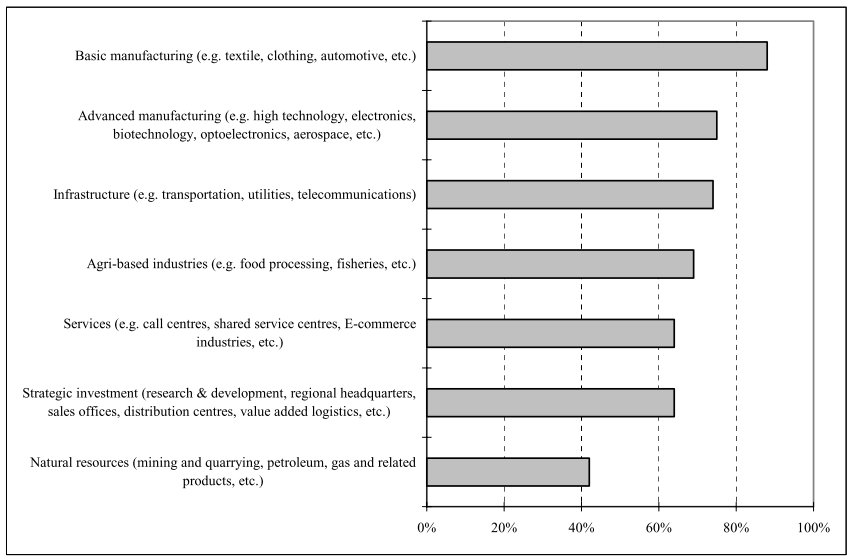
\includegraphics[width=\textwidth,keepaspectratio]{../figure/IPA_target_industries}
  \caption[Target industries by IPA around the world.]{Target industries by IPAs
    around the world. Because of the image building aspect of investment
    promotion, almost all IPAs say that they want to attract ``manufacturing,''
    ``advanced manufacturing,'' and ``infrastructure.'' Therefore, using what is
    listed as investment priorities may not be a reliable way to measure
    countries' preference for FDI. Source: \citet{UNCTAD2001}}
  \label{fig:IPA_target_industries}
\end{figure}

In sum, differentiating FDI by sectors only gives us a crude typology of FDI. We
can address this challenge using firm-level data, giving us information on not
only a firm's sector but also its operational characteristics, such as research
and development (R\&D) expenditure or export intensity. These measures are
firm-specific and get closer to what countries are looking for in FDI projects.
Using R\&D expenditure or export intensity as firms' characteristics in the
two-sided matching model, I will be able to estimate countries' preferences for
these traits.

\section{Measuring MNCs' activities}

As \citet{Kerner2014} argues, the IPE literature on FDI is a bit of a misnomer.
Political scientists are rarely interested in FDI \textit{per se}---rather, they
are interested in the activities of MNCs, which in turn, affect other important
issues such as nation-state autonomy \citep{Mosley2005}, economic development
\citep{Moran1998}, labor standards \citep{Mosley2007}, and environmental
policies \citep{Prakash2007}. However, while the theory involves MNCs as the
central actor in the causal mechanism, the empirics often uses FDI flow as the
variable of interest. These two concepts---the level of MNCs' affiliate
activities in a country and FDI inflow into a country---are not the same.

Consider the definition of FDI from UNCTAD, the main producer of FDI data widely
used by researchers:

\begin{quote} FDI has three components: equity capital, reinvested earnings and
  intra-company loans.
  \begin{itemize}
  \item Equity capital, i.e. the foreign investor’s purchase of shares of an
    enterprise [in the host country].
  \item Reinvested earnings, i.e. the foreign investor’s share \ldots of
    earnings not distributed as dividends by affiliates, or earnings not
    remitted to the foreign investor.
  \item Intra-company loans between direct investors and affiliate enterprises.
  \end{itemize} \citep[245]{UNCTAD2007}
\end{quote}

In essence, FDI data captures the amount of capital that crosses border. It is a
poor proxy for the scale of MNCs' activities in the host country because it
overlooks important components of MNCs' activities while including components
that are only relevant for balance of payment statistics
\citep{Beugelsdijk2010}.

Consider the argument that FDI is the driver for the diffusion of labor
standards across countries. \citet{Mosley2007} theorizes that FDI can have this
effect through three channels. First, MNCs may pressure the host government for
better rule of law and social programs. For MNCs to be able to effectively exert
this pressure, they must prove themselves valuable to the government by
providing jobs or tax revenue. Both of these factors are tenuously related to
the amount of foreign capital inside the host country. Indeed, an MNC can employ
thousands of employees, pay millions in tax, but show up as a net 0 on FDI flow
data because the profit is repatriated to the foreign investor or through
intra-company loans.\footnote{The issue of intra-company loans is particularly
  fraught with issues because companies very frequently use intra-company loans
  to get out of paying tax in a country. These loans will be recorded on the
  book as a massive outflow, even though the MNC still has a large presence on
  the ground.} The scale of MNCs' operation is further understated because FDI
statistics does not take into account capital raised locally. Also not included
is the superior productivity of MNCs, which acts as an important multiplier when
translating the amount of capital to the amount of output.

Second, scholars argue that MNCs may bring along best practices for workers'
rights and spread it to local firms. If this spillover effect happens via
competition, i.e. MNCs providing better working condition and forcing local
firms to compete, then MNCs must employ a lot of labor for this effect to be
noticeable. Or if the spillover happens via demonstration, then MNCs must form a
lot of linkages with local firms, as suppliers and buyers, for the diffusion of
norms to happen. Both the size of the labor force and the type of linkages with
the local economy are not captured by FDI flow statistics.

Third, scholars argue that MNCs may care more about labor quality than its cost,
and thus may invest in higher wages, better benefits, or more training. Once
again, for this effect to be noticeable, the MNC's industry, size of labor
force, and investment in productivity all matter a lot more than how much
capital it brings in and out of the country. In addition, non-equity
transactions between the parent company and the subsidiary, such as transfer of
knowledge, technology, and management practices, are not counted in FDI flow
statistics, thus excluding another component that is arguably much more
important to labor quality than the amount of capital.\footnote{These issues are
  not isolated to studies of FDI and labor standards, but are common to the
  whole IPE literature of the effect of FDI on policy convergence, such as
  environmental policies \citep{Prakash2007}.}

This mismatch between theory and empirics may also be a reason behind the
unsettled debate on the effect of FDI on poverty reduction. Scholars have
theorized that FDI can lead to economic development through three channels:
cheaper goods, technology transfer, and tax revenue. Once again, the causal
variable in the second and third channels is the scale and the type of MNCs'
activities in the host country, not necessarily the amount of capital crossing
the border. Indeed, productivity spillover is highly conditional on the
technological capability of the MNC and whether it forms thick linkages with the
local suppliers. The effect of FDI via tax revenue is also fraught with issues,
as MNCs frequently use intra-company transactions to artificially reduce book
profit and get out of paying tax \citep{Malesky2015c}.\footnote{These tactics
  are called ``transfer pricing,'' and can include tactics such as charging for
  internal intellectual properties and services whose price can be set
  arbitrarily by the firm} Since FDI flow statistics do not record these
intra-company transactions, it is not surprising that researchers reach the
confusing conclusion that FDI does not generate tax revenue.

What about studies that use FDI as the dependent variable, and are thus perhaps
interested in the flow of capital in and of itself?\footnote{Arguably, political
  scientists are not interested in the flow of capital in and of itself, but
  because of its implications for development, state autonomy, and other effects
  on policy. The discussion above has shown how problematic it is to study these
  effect of FDI using FDI flow data.} The vast majority of these studies on the
determinants of FDI flow rely on the ``obsolescing bargain'' model. Originally
developed by \citet{Vernon1971}, the model is so named because the bargaining
dynamics between the MNC and the host government changes over time, initially
favoring the MNC and gradually tips towards the host government as the MNC
commits more fixed capital on the ground. Indeed, knowing that it is costly for
the MNC to uproot its increasingly large and immobile operation, the host
government can unilaterally alter the original bargain, most egregiously by
expropriating the MNC's asset and profit, but more often via ``creeping
expropriation,'' e.g. increased tax or tougher regulation \citep{Li2009a}.
Political economists argue that MNCs are acutely aware of the ``obsolescing
bargain,'' and thus prefer to invest in countries whose governments can make a
credible commitment that they will not alter the original deal. This argument
translates into a large literature claiming that MNCs prefer countries with
democratic accountability \citep{Jensen2003}, a federal system
\citep{Jensen2005}, membership in international trade agreements
\citep{Buthe2008}, less political risk \citep{Beazer2011, Graham2010}, or more
veto points \citep{Choi2008}.

The linchpin of this argument is the assumption that FDI capital is illiquid and
cannot be quickly removed from the host country at will. This assumption is not
fully warranted. According to the US Bureau of Economic Analysis (BEA)'s 2004
survey, 43\% of US MNCs' balance sheet comprises of liquid assets that can be
liquidated within one year under normal operating situations. Among the 57\% of
the balance sheet that are illiquid, 24\% are ``other non-current assets,''
which include non-tangible assets like brand names, trademarks, and
patents---some of which are not expected to be liquidated but can be easily
removed from host countries. Only another 24\% of the balance sheet is made up
of physical capital, i.e. Plant, Property, and Equipment (PPE), which cannot be
easily moved and match most closely to what we have in mind as the ``illiquid
capital'' in the obsolescing bargain model \citep[113]{Kerner2014a}. Since FDI
flow data does not distinguish between liquid and illiquid capital, it is
suspect to use FDI flow data to test the ``obsolescing bargain'' argument,
calling into questions the entire literature on the political determinants of
FDI.

Besides the conceptual mismatch between FDI flow and MNCs' activities, from a
statistical standpoint, this measurement error may also be a contributing factor
to why there is little consensus in the FDI literature. Even if the measurement
error is random, it will inflate the standard error of our estimate when FDI is
the dependent variable, and bias our estimate towards 0 when FDI is the
independent variable. These effects may explain \citet{Jensen2012}'s surprising
finding that lower corporate tax rate does not lead to more FDI flow, or the
mixed empirical evidence for the relationship between FDI and development
\citep[108]{Mold2004}.

Even more worryingly, the measurement error is unlikely to be
random.\footnote{See \citet{Gallop2017} for a recent and more comprehensive
  discussion of measurement error in political science research.} For example,
the amount of locally raised capital---an important source of capital for MNCs
yet not captured in FDI flow data---is likely to correlate with how developed
the local capital market is or how wildly the exchange rate fluctuates.
Similarly, repatriated earnings, which does not necessarily indicate reduced
MNCs' activities but is recorded as an outflow in FDI flow data, is likely to
correlate with the tax rate of not only the host country but also other tax
havens that the MNC may have an affiliate in.

To deal with this measurement error problem, scholars have attempted to use
measurements that are closer to the theory than FDI flow. Given that political
scientists are often interested in MNCs' activities, recent work emphasizes
using MNCs' operational data directly. These firm-level datasets allow
researchers to measure directly the quantities of interest. For example,
re-visiting \citet{Li2009a}'s hypothesis that democracies are more attractive to
MNCs, \citet{Kerner2014} uses data on US MNCs' fixed capital expenditure to more
precisely test the relationship between democratic institutions and FDI
\textit{illiquid} capital, not just FDI in general. The author finds that there
is no relationship between democratic institutions and FDI flow, but there is a
positive relationship between democracy and MNCs' fixed capital expenditure,
confirming the theoretical expectation. Similarly, when \citet{Jensen2008a}
re-examines whether MNCs favor democratic regimes because they pose less
political risk, the author avoids using FDI flow and relies on price data of
political risk insurance agencies instead.\footnote{Scholars in other areas of
  IPE are also paying more attention to the issue of measurement error and the
  mismatch between empirics and theory, e.g. \citep{Karcher2013}.}


\section{Next steps}

In sum, the current FDI literature would benefit from focusing on countries'
preference for FDI, distinguishing types of FDI, and using firm-level
operational data instead of aggregate FDI flow statistics. While the theoretical
needs are clear and firm-level data has become more abundant in recent years,
political scientists have not developed a model to estimate this data structure
appropriately.\footnote{Examples of firm-level data include the US Bureau of
  Economic Analysis (BEA)'s survey of all US firms abroad, Tokyo Keizai's
  Overseas Japanese companies database (\textit{Kaigai Sinshutsu Kigyou
    Souran}), World Bank's Enterprise Survey, and Orbis database of companies
  worldwide.}

Very often, given the data structure of a set of firms interacting with a set of
countries, scholars resort to a dyadic-based analysis perhaps due to its being a
familiar tool. In such analysis, the unit of observation is a firm-country dyad,
and the model used is typically OLS regression. Each dyad is assumed to be
independent of each other, and any bias caused by interdependency is fixed via
post-estimation procedures, such as clustered standard errors \citep{Dorff2013}.
Unfortunately, this dyadic approach is patently inappropriate to analyze MNCs'
investment location. Indeed, once a firm chooses to invest in a country, it is
by definition not investing in another. Therefore, the values of firm-country
dyads deterministically constrain one another and cannot be modeled as
independent draws from a common distribution.\footnote{As a recent example,
  \citet{Arel-Bundock2017} uses Orbis, a global dataset of firms, to study the
  location decision of MNCs. The author uses random forest, a non-parametric
  machine learning approach, to predict whether an investment materializes for
  each of MNC-country dyad. However, because the predictors in the random forest
  model are dyad-specific, this approach cannot model interactions between
  dyads. In addition, since random forest does not produce interpretable
  coefficients, this black-box approach does not allow us to understand the
  preference of actors, how these preference are correlated with other
  characteristics, and how they may evolve over time.}

I propose using the two sided matching model to simultaneously address all of
these three issues in the literature. This approach models the matching process
explicitly, thus taking into account the dependency across dyads. The matching
process is made up of actors maximizing their utility functions---therefore, we
gain direct insight into what countries and MNCs value the most. Finally, the
model uses firm-level operational data, circumventing the measurement error
problem of aggregate FDI flow statistics. In the next chapter, I describe in
details how the two-sided matching model is set up and estimated.

%%% Local Variables:
%%% mode: latex
%%% TeX-master: "AnhLe_dissertation.tex"
%%% End: